% !TEX encoding = UTF-8 Unicode
\documentclass[10pt]{amsart}

%%% MY PACKAGE
\usepackage{mysetup}

\allowdisplaybreaks 

\begin{document}
	
	\title{Assignment No. 2: Advanced Methods}
	\author{Studend ID: 10729579}
	\maketitle
	
	\vspace{-0.3cm}
	\setcounter{secnumdepth}{0}
	\section{Introduction}
		\noindent We are supposed to price a bond contract whose terminal condition is given by
%%% TERMINAL CONDITION OF THE BOND PRICE 
\begin{equation}
	V(S,T) = \max \left(F, RS\right).
\end{equation}

Moreover, the issuer of the bond pays out a continuous coupon at the rate of 
\begin{equation}
	K(t) = C \exp{-\alpha t},
\end{equation}
for $\alpha$ and $C$ of his choosing. 

The risk-neutral process followed by underlying stock price is given by
\begin{equation}
	\d S = \kappa \left(\theta(t)  - S\right)\d t + \sigma S^\beta \d W,
\end{equation}
with $\kappa$ being the mean reversion rate, $\beta$ the elasticity of variance in the market, and the function $\theta$ is given by
\begin{equation}
	\theta(t) = (1+\mu)X\exp{\mu t},
\end{equation}
where $X$ and $\mu$ are constant model parameters that can be determined from the market, reflecting the dividend payout of the firm.

The market value $V(S,t)$ of this contract satisfies the following PDE
\begin{equation}\label{general_pde}
	\partial_t V + \frac{1}{2}\sigma^2 S^{2\beta}\partial_{SS}V + \kappa (\theta(t) - S)\partial_SV - rV + C\exp{-\alpha t} = 0,
\end{equation}
where its boundary conditions are given by
\begin{equation}\label{pde_S0}
	\partial_t V + \kappa \theta(t) \partial_S V - rV + C\exp{-\alpha t} = 0, \doublequad \text{ at } S= 0,
\end{equation}
and
\begin{equation}
	V(S,t) = S A(t) + B(t), \doublequad \text{ as } S\to\infty,
\end{equation}
for $A$ and $B$ some functions to be derived.
	
	%& FIRST TASK: EUROPEAN OPTIONS
	\setcounter{secnumdepth}{4}
	\section{European Options}
		\subsection{Derivation of boundary condition for large $S$}
			%& TASK 1: EUROPEAN OPTIONS
\noindent We are told to derive the boundary conditions for (\ref{general_pde}). To do so, we are assuming that 
%%% BOUNDARY CONDITIONS: ASSUMPTION FOR THE SOLUTION OF THE PDE 
	\begin{equation}\label{boundary_condition}
		V(S, t) = S A(t) + B(t) \doublequad \text{ as } S\to \infty,
	\end{equation}
for some functions $A$ and $B$ which solve the approximate problem
%%% THE PDE 
	\begin{equation}\label{pde}
		\partial_t V + \kappa (X - S) \ \partial_S V - rV + C \exp{-\alpha t} = 0
	\end{equation}
obtained after taking $S\to\infty$ in (\ref{general_pde}). We must firstly note~that
	\begin{equation}\label{derivatives}
		\partial_t V (S, t) = S A'(t) + B'(t), \doublequad \text{ and } \doublequad \partial_S V = A(t),
	\end{equation}
to further substitute (\ref{derivatives}) in (\ref{pde}) and get
	\begin{equation}\label{calc1}
		\begin{aligned}
			S A'(t) + B'(t) + \kappa (X - S) A(t) - r \left[ S A(t) + B(t)\right] + C\exp{-\alpha t} = 0.
		\end{aligned}
	\end{equation}

Since the solution is of the form (\ref{boundary_condition}), we may arrange (\ref{calc1}) into something of the same form, that is,
	\begin{equation}\label{calc2}
		\begin{aligned}
			S \left[A'(t) - (\kappa + r) A(t) \right] + \left[ B'(t) + \kappa X A(t) - rB(t) + C\exp{-\alpha t}\right] = 0,
		\end{aligned}
	\end{equation}
which is equivalent to solve
	\begin{equation}
		\begin{cases}
			A'(t) &=  (\kappa + r) A(t) \\
			B'(t) &= rB(t)  - f(t) \\
		\end{cases},
	\end{equation}
where $f(t) = \kappa X A(t) + C\exp{-\alpha t}$.

The first equation gives us that $A(t) = A_T \exp{-(\kappa + r)(T-t)}$, with 
$
A_T \overset{\text{\tiny def}}{=} A(T) \to R,
$ 
as $S\to\infty$. Hence, 
\begin{equation}\label{A}
	A(t) = R\exp{-(\kappa + r)(T-t)}
\end{equation} 

On the other hand, second equation gives us that $B$ is of the form $B(t) = C(t) \exp{-r (T-t)}$, $C(T) = B(T)$, where $C(t)$ is to be derived. Differentiating $B(t)$ and rearranging terms we get
%%% ODE FOR THE "CONSTANT" MULTIPLYING B
	\begin{equation}\label{C_ode}
		C'(t) = - \exp{r(T-t)}f(t), 
	\end{equation}
with $  B_T \overset{\text{\tiny def}}{=} B(T) $, which is zero for large $S$, i.e.,
	\begin{equation}\label{C_ode_sol}
		 C(t) 	= B_T + \int_t^T \exp{r(T-s)}f(s)\d s,
	\end{equation}
which implies that (see Appendix \ref{app_ODE_C})
	\begin{equation}
		C(t) = B_T + {X R}  \left[1 -  \exp{-\kappa(T-t)}\right]- \frac{C}{r+\alpha}\exp{rT}\left[\exp{-(r+\alpha)T}-\exp{-(r+\alpha)t}\right]
	\end{equation}

Therefore, for $S$ sufficiently large we obtain (see Appendix \ref{app_ODE_C}),
	%%% B(t) 
	\begin{equation}\label{B}
			B(t)  = {2X R}\exp{-\left(r+\frac{\kappa}{2}\right)(T-t)}\sinh\left(\frac{\kappa}{2}[T-t]\right)- \frac{C}{r+\alpha}\exp{rt}\left[\exp{-(r+\alpha)T}-\exp{-(r+\alpha)t}\right]
	\end{equation}

Finally,
	%%% VALUE FUNCTION WHEN S TENDS TO INFINITY
	\begin{equation}\label{boundary_formula}
		V(S,t) = SR  \ \exp{-\kappa_r(T-t)} +  {2X R}\exp{-\frac{1}{2}\left(r-\kappa_r\right)(T-t)}\sinh \frac{\kappa}{2}(T-t)- \frac{C}{\alpha_r}\exp{rt}\left[\exp{-\alpha_r T}-\exp{-\alpha_r t}\right],
	\end{equation}
	where $\kappa_r \defi \kappa + r$, and $\alpha_r \defi  \alpha + r.$

		\subsection{Crank Nicolson Scheme}
			As we are told to do, we have used the Crank-Nicolson scheme to calculate the value of the option.

To do so, we have calculated an analytic solution for $V$ both when $S=0$ and $S$ becomes large, in order to set the boundary conditions up, i.e., $a[0], b[0], c[0], d[0]$ and $a[\texttt{m\_J}], b[\texttt{m\_J}], c[\texttt{m\_J}], d[\texttt{m\_J}]$, with \texttt{m\_J} being the member variable of the class \texttt{CCrackNicolson} which can be found in the files \texttt{CCrackNicolson.cpp} and \texttt{CCrackNicolson.h}, and which gives us the distance between the stock prices of the grid, i.e.,  $\texttt{m_dS} = \texttt{m_Smax} / \texttt{m_J}$ . The derivation of $V(S=0, t)$ using the method of characteristics for first-order partial differential equations can be found in the Appendix \ref{app_bound_V_S0}:
\begin{equation}\label{V_S0}
	V(S=0,t) =  F \exp{-r(T-t)} + \frac{C}{r+\alpha} \exp{-\alpha T}\left( \exp{\alpha (T-t)} -\exp{-r(T-t)} \right).
\end{equation}

On the other hand, the derivation of the coefficients can be found in the Appendix \ref{app_coeff_CrankNic}, and are given by 
\begin{equation}
	\begin{aligned}
		a(j) &= -\frac{1}{4}\sigma^2j^{2\beta}(\Delta S)^{2(\beta -1) }+ \frac{\kappa}{4}\left[\frac{\theta(\Delta t)}{\Delta S} - j\right] \\
		b(j) &= \frac{1}{\Delta t} + \frac{r}{2} + \frac{1}{2}\sigma^2 j^{2\beta}(\Delta S)^{2(\beta -1) }\\
		c(j) &=  -\frac{1}{4}\sigma^2j^{2\beta}(\Delta S)^{2(\beta -1) } - \frac{\kappa}{4}\left[\frac{\theta(\Delta t)}{\Delta S} - j\right]\\
		d(i,j)&=\left(\frac{1}{4}\sigma^2 j^{2\beta}(\Delta S)^{2(\beta -1) } - \frac{\kappa}{4}\left[\frac{\theta(\Delta t)}{\Delta S} - j\right]\right)V_{i+1,j-1}\\
		&+ \left(\frac{1}{\Delta t } - \frac{1}{2}\sigma^2 j^{2\beta}(\Delta S)^{2(\beta -1) }  - \frac{r}{2}\right)V_{i+1,j}\\
		&+ \left(\frac{1}{4}\sigma^2 j^{2\beta}(\Delta S)^{2(\beta -1) }+ \frac{\kappa}{4}\left[\frac{\theta(\Delta t)}{\Delta S} - j\right]\right)V_{i+1,j+1} + C \exp{-\alpha \Delta t}.
	\end{aligned}
\end{equation}
for all $0< j < \texttt{m_J}$.

For $j=0$ and $j = \texttt{m_J}$ we set $a[0] = c[0] = a[\texttt{m\_J}] = c[\texttt{m\_J}] =  0$ and $b[0] = b[\texttt{m\_J}] = 1$ because we have an analytic solution for both cases. More precisely, in the $i$th step, $\texttt{d[0]} = \texttt{V_S0}[(i + 0.5) * \texttt{m_dt}]$, where $\texttt{m_dt} = \texttt{m_T} / \texttt{m_I}$, with $m_T$ the time to maturity (in our case is $T=3$) and $\texttt{m_I}$ is the number of time steps we want in our grid. The function $\texttt{V_S0}$ can be found in the class $\texttt{CConvertibleBonds}$ within the files \texttt{Convertiblebonds.cpp} and \texttt{ConvertibleBonds.h}.

Analogously, in the $i$th step, $d[\texttt{m_J}] = \texttt{V_Smax}(\texttt{m_Smax, (i + 0.5) * \texttt{m_dt}})$, where he function $\texttt{V_Smax}$ can be found in the class $\texttt{CConvertibleBonds}$ within the same two files.

In other words, for all $i$,
\begin{equation}
	\begin{aligned}
		d(i,0) &= F \exp{-r(T-(i + 0.5) \Delta t)} + \frac{C}{r+\alpha} \exp{-\alpha T}\left( \exp{\alpha (T-(i + 0.5) \Delta t)} -\exp{-r(T-(i + 0.5) \Delta t)} \right),\\
		d(i,J) &= Smax \ A((i + 0.5) \Delta t) + B((i + 0.5) \Delta t),
	\end{aligned}
\end{equation}
where $A$ and $B$ are the functions given in (\ref{A}) and (\ref{B}).



		\subsection{Value of the option at $t=0$ as a function of $S$.}
			In this task we are aim to find the value of the option, $V(S,t)$ as a function of the underlying asset price $S$ at $t=0$, i.e., $V(S,t=0)$. In order to so, we are given two pairs of specific values of $\beta$ and $\sigma$. 
\begin{enumerate}[wide, labelindent=1cm]
	\item $\beta=1$ and $\sigma = 0.381$, and all other parameters as standard.
	\item $\beta=0 0.808$ and $\sigma=0.66$, and all other parameters as standard.
\end{enumerate}
\vspace{-0.3cm}
\begin{figure}[htbp]
	\centering
	\captionsetup{width=.5\linewidth}
	\begin{subfigure}[b]{0.49\textwidth}
		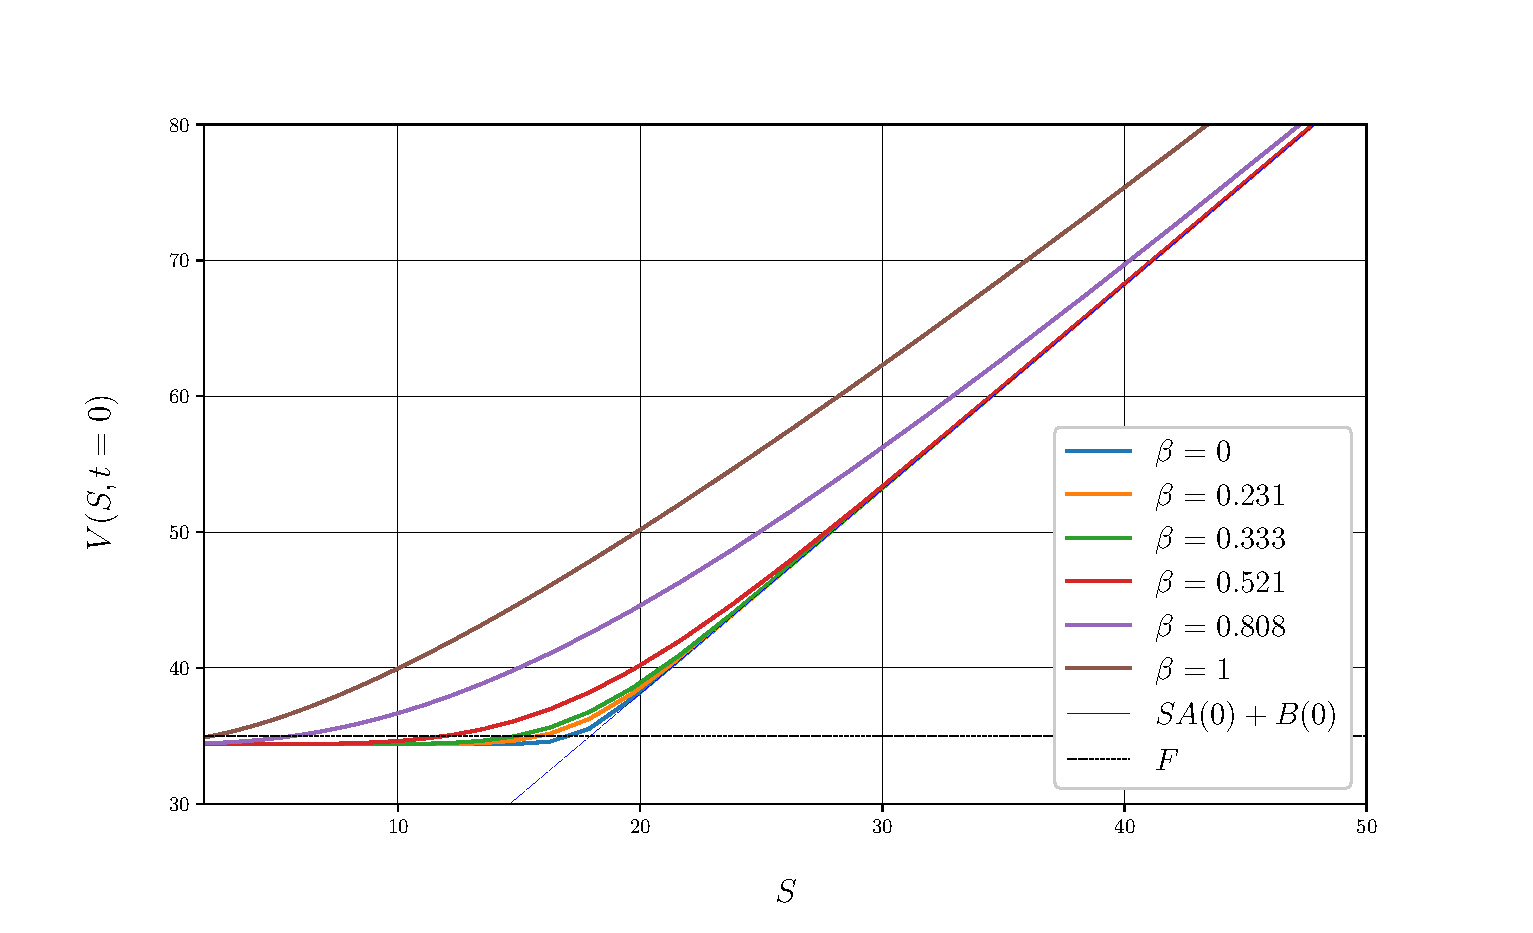
\includegraphics[width=\textwidth]{img/Q1/ComparisonDifferentBetas_sigma06600.eps}
		\captionsetup{width=.8\linewidth}
		\caption{Value of the option for different $\beta$ as $S$ becomes larger with $\sigma = 0.381$.}
		\label{changingBeta}
	\end{subfigure}
	\begin{subfigure}[b]{0.49\textwidth}
		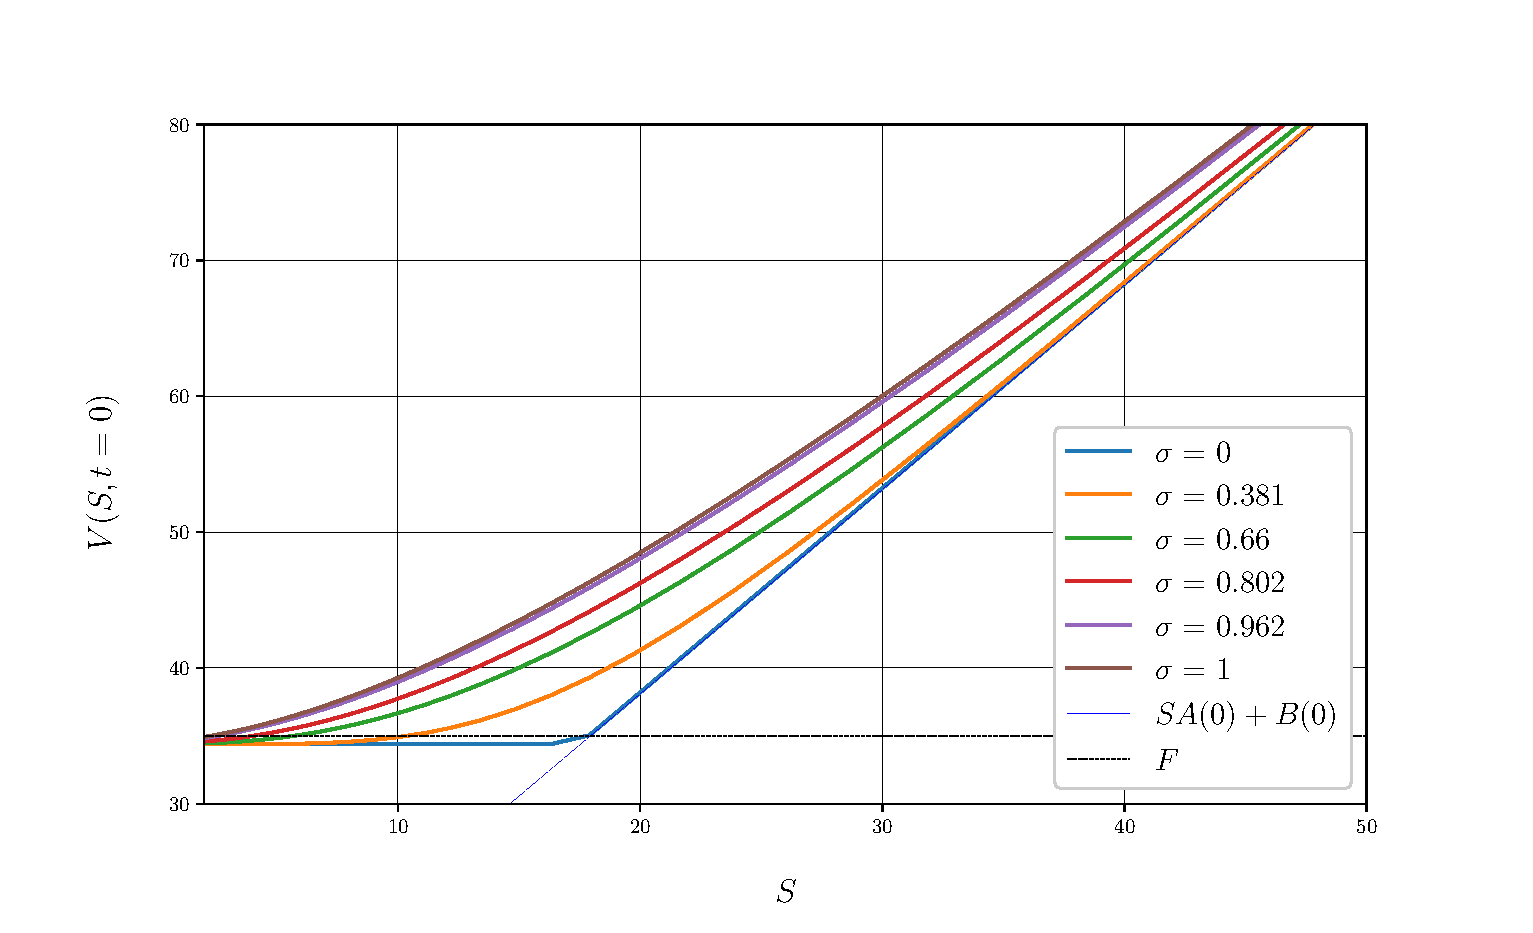
\includegraphics[width=\textwidth]{img/Q1/ComparisonDifferentSigmas_beta0808.eps}
		\captionsetup{width=.8\linewidth}
		\caption{Value of the option for different $\sigma$ as $S$ becomes larger with $\beta=0.808$.}
		\label{changingSigma}
	\end{subfigure}
	\caption{Value of the option as $S$ becomes larger for different parameters.}
	\label{S_larger}
\end{figure}
\vspace{-0.3cm}
The idea is to see what happens when $\beta$ and $\sigma$ are changed, so firstly let's plot some graphs with a few values of $\beta$ and $\sigma$. We have chosen six values for both parameters from $0$ to $1$ (including them). In Figure \ref{changingBeta}, $\sigma$ is fixed, whilst $\beta$ is fixed in Figure \ref{changingSigma}. But firslty we are trying to understand theoretically what's going on. On the one hand, both $\beta$  and $\sigma$ contribute to the term 
\begin{equation}
	\frac{1}{2}\sigma^2S^{2\beta}\partial_S^2 V.
\end{equation}

Moreover, note from (\ref{general_pde}) that
\begin{equation}
	V = \frac{1}{r}\left(\partial_t V + \frac{1}{2}\sigma^2 S^{2\beta}\partial_{SS} V + \kappa\left(\theta(t) - S\right)\partial_S + Ce^{-\alpha t}\right);
\end{equation}
which means that, when all of the parameters are the same but not $\beta$ and $\sigma$, then we can understand $V(S,t)$ as
\begin{equation}\label{useful}
	V = \frac{1}{2r}\sigma^2 S^{2\beta}\partial_{SS} V + \text{other}.
\end{equation}

On the other hand, we know that when $S$ becomes larger, $V(S,t)$ tends to $S A(t) + B(t)$, so the contribution of $\beta$ and $\sigma$ is significant when $S$ is somehow small. Moreover, it is obvious from (\ref{useful}) that $V$ becomes smaller as $\sigma$ and $\beta$ becomes smaller. Particularly, when $\beta \to 0$, then
\begin{equation}
	V \to  \frac{1}{2r}\sigma^2\partial_{SS} V + \text{other};
\end{equation}
and, when $\sigma\to 0$, 
\begin{equation}
	V \to  \text{other},
\end{equation}
and the contribution of the second derivative with respect of $S$ is null, i.e., it's (locally) linear on $S$ (tending to $F$ for small $S$). This is coherent with Figure \ref{S_larger}, in which we can see how the value of the option flattens before the cross of $F$ and $S A(0) + B(0)$, i.e., when
\begin{equation}
	S^* = \frac{F-B(0)}{A(0)} = 17.94670.
\end{equation} 

This means that when $S < S^*$, then $V(S,0) \to F$ as $\sigma, \beta\to0$. Intuitively speaking, $\sigma$ is the volatility of the process, so the larger the sigma, the larger the random fluctuation from the Brownian Motion. In some sense, it increases the randomness of the stock price. On the other hand, $\beta$ can be understood as the elasticity of the stock price, meaning that $\sigma S^\beta$ is the instantaneous volatility of the stock price, i.e., 
\begin{equation}
	\frac{\partial_S \left(\sigma S^\beta\right)}{\sigma S^{\beta}/S} =\frac{\sigma \beta S^{\beta-1}}{\sigma S^{\beta-1}} = \beta,
\end{equation}
which means that it is the percentange of change in instantaneous volatility as $S$ changes. If $\beta < 1$, the volatility increases as the stock price decreases, and viceversa, but not monotonically: since $\sigma S^{\beta}$ is a concave function on $S$, then de increasing is faster for smaller $S$.

\begin{figure}[htbp]
	\centering
	\captionsetup{width=.5\linewidth}
	\begin{subfigure}[b]{0.49\textwidth}
		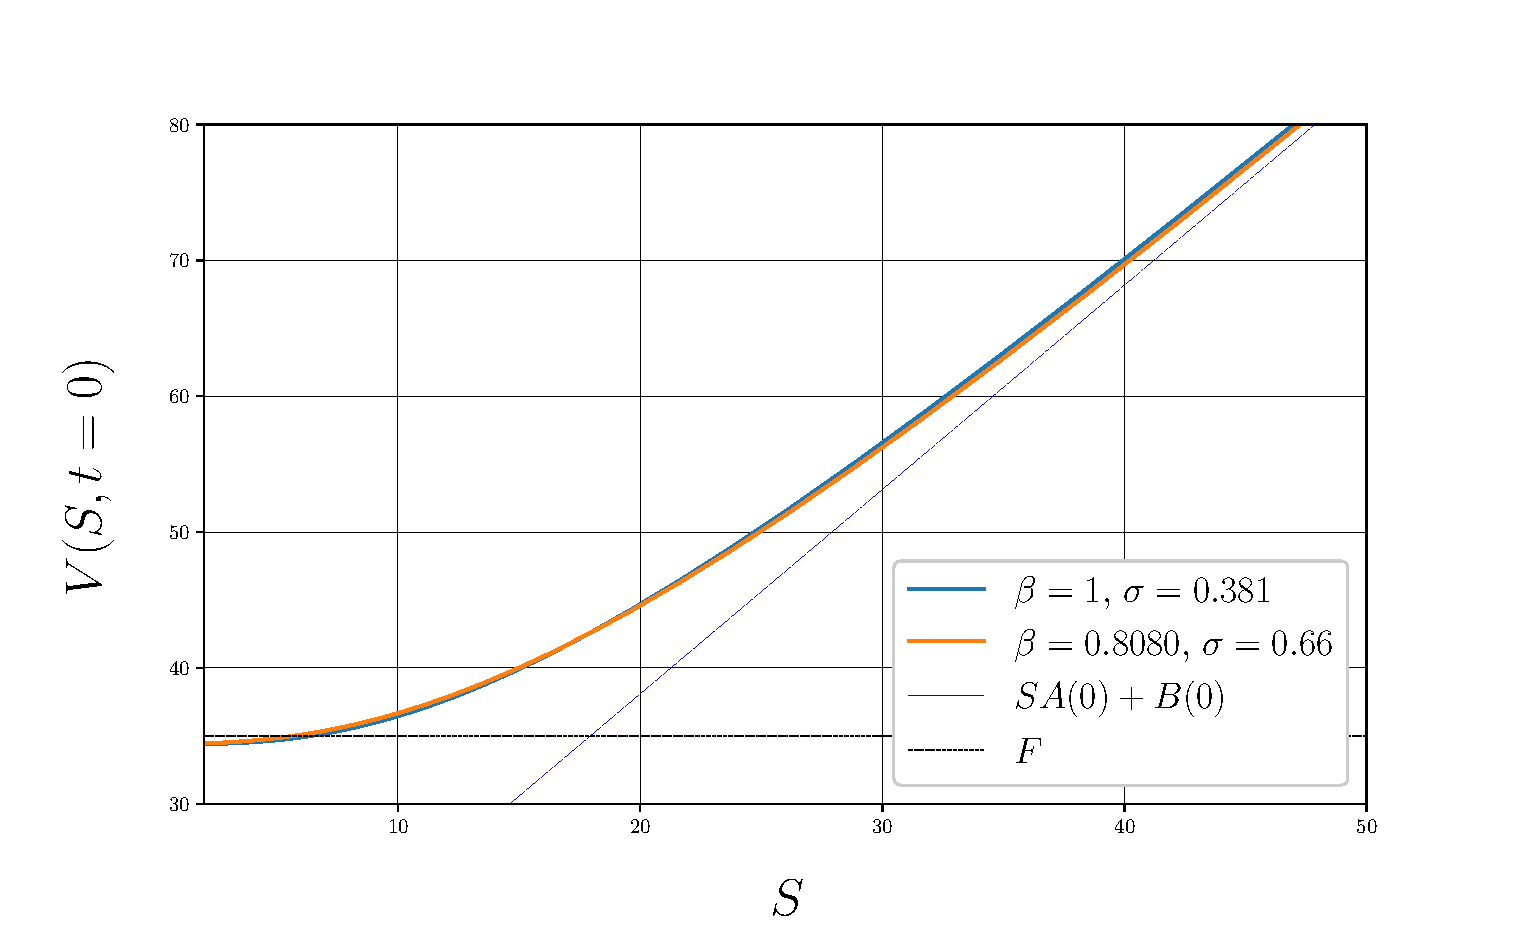
\includegraphics[width=\textwidth]{img/Q1/ComparisonGivenBetaAndSigma.eps}
		\captionsetup{width=.8\linewidth}
		\caption{Value of the option for different $\beta$ as $S$ becomes larger with $\sigma = 0.381$.}
		\label{withoutZoom}
	\end{subfigure}
	\begin{subfigure}[b]{0.49\textwidth}
		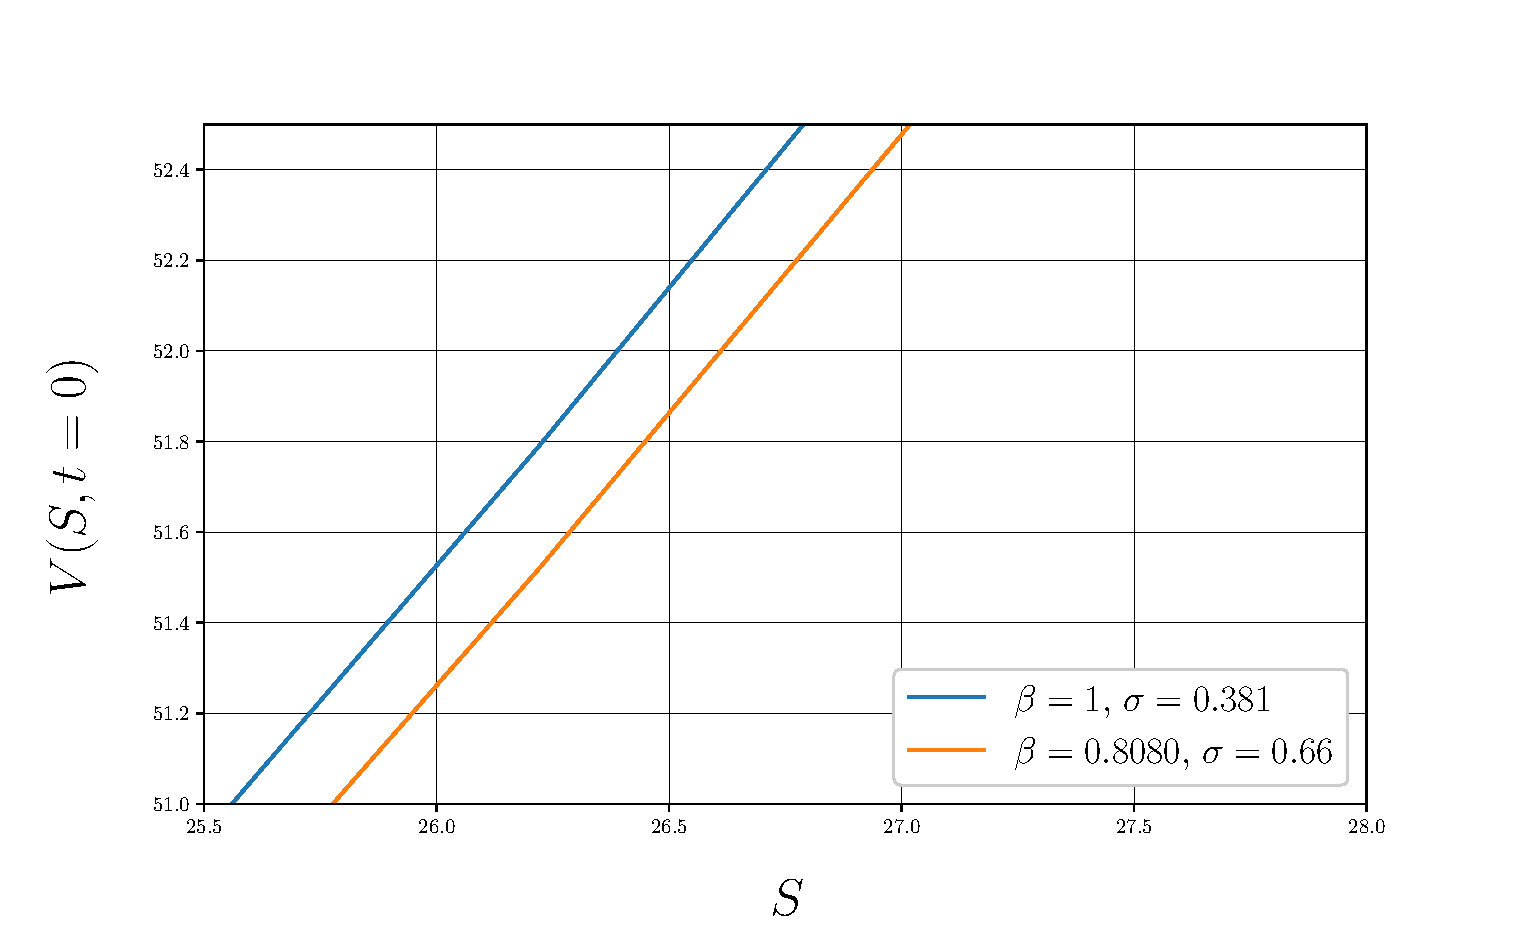
\includegraphics[width=\textwidth]{img/Q1/ComparisonGivenBetaAndSigmaZoom.eps}
		\captionsetup{width=.8\linewidth}
		\caption{Value of the option for different $\sigma$ as $S$ becomes larger with $\beta=0.808$.}
		\label{withZoom}
	\end{subfigure}
	\caption{Value of the option as $S$ becomes larger for different values of parameters $\beta$ and $\sigma$.}
	\label{StudyingBetaSigma}
\end{figure}

In particular, we are told to study the option option value when $\beta=1$ and $\sigma = 0.381$ and $\beta=0.808$ and $\sigma=0.66$. As we can see in Figure \ref{withoutZoom}, the results are nearly the same, just separated by a difference of $0.2$ (see the Figure \ref{withZoom}). This means that a relatively low $\sigma$ is compensated with a relatively big $\beta$ and viceversa. Moreover, all the solutions will converge to the same line, because  (\ref{boundary_formula}) does not depend on $\beta$ and $\sigma$. Hence, the role of $\beta$ and $\sigma$ is just to determine how fast the solution converges to $SA(0) + B(0)$ for $S>S^*$ and how plattened it is when $S<S^*$.



		\subsection{Value of the option when $S_0=17.38$.}
			In this task we have to find the value of the option when $S_0 = 17.38$, and $\beta = 0.808$ and $\sigma  = 0.66$. To do so, we set a squared-grid, i.e., $\texttt{m_J} = \texttt{m_I} = N$ and obtain different values (first column of the next tables). From a first sight, we can roughly see that the value of the option when $S_0 = 17,38$ is around $42.05\pm10^{-2}$. However we would like to see how much we could improve our result to get more digits of precision. This can be done by increasing $S_{max}$. The idea is to have $S_0$ within the points of the grid, although we can make use of Lagrange Interpolation (of different degrees) to make sure we have a correct result. However, this would add some errors, and it is desiderable to avoid them. The idea is therefore to make sure that there exists a $j^*$ such that $S_0 = j^* \Delta S$, where $\Delta S = S_{max} / J$. Therefore, $j^* = \frac{S_0 J}{S_{max}}$ but, in our case, we have that $X = S_0$, so an easy way to make $J$ an integer is to take $S_{max} = k X$. This would imply that $J =  k j^*$ for some integer $k$. On the other hand, in order to study the convergence, we must iterate the method with different $J$. To do so, we have done a loop ``\texttt{for (int n=nMin; n<=nMax; n*=incr)}'' with $\texttt{nMin=3, nMax=50000, incr=2}$ (they could have been different) and with $\texttt{I=J=n*ceil(Smax/S0)=n*k}$. We can see an example in Table \ref{table1}.

\begin{table}[h!]\scriptsize
	\setlength{\tabcolsep}{5pt}
	\renewcommand{\arraystretch}{1.3}
	\begin{tabular}{c|ccccccccc}
		\hline\addlinespace[0.1cm]
		I=J			& 48	& 96 & 192 & 384 & 768 & 768 & 1546 & 2072 & 6144 \\
		$V(S_0,0)$ & 41.8408512 & 42.004891854 & 42.04124385 & 42.04867403 & 42.04973806 & 42.049609 & 42.04957 & 42.0495647 & 42.049562 
       \\\addlinespace[0.1cm]
		\hline
	\end{tabular}
	\vspace{0.3cm}
	\captionsetup{width=.55\linewidth}
	\caption{Values when increasing $\texttt{m_I}$ and $\texttt{m_J}$, Lagrange Interpolation of degree $16$ and $S_{max} = 8X$.}\label{table1}
\end{table}
\vspace{-0.6cm}
In order to improve our results and get more efficiency using a lower $J$, we can study the convergence of our values to further use Richardson Extrapolation (maybe more than one time). The ratios of the difference between results\footnote{Given three values $v_1$, $v_2$, $v_3$, we define the ratio between their differences as $\frac{v_2-v_1}{v_3-v_2}$. Since the convergence of Crank Nicolson method is $\mathcal{O}((\Delta S)^2, (\Delta t)^2)$, then we expect this ratio to be $4$, because the increments are produced by doubling $J$.} can be found in Table \ref{table2}.

\begin{table}[h]\scriptsize
	\setlength{\tabcolsep}{8pt}
	\renewcommand{\arraystretch}{1.3}
	\begin{tabular}{r|rrrrrrrrrr}
		\hline\addlinespace[0.1cm]
		$V(S_0,0)$ & 4.51256 & 4.89249 & 6.98301 &  8.26535 & 3.47294 & 4.95559 & 2.69404 & 9.72845 & 0.97506 & \\
		I Extrap & 2.80979 & 2.08924 & 2.01019 & 80.82043 & 2.73326 & 1.97126 & 2.21787 & 1.84651 & 2.29676 &          \\\addlinespace[0.1cm]
		\hline
	\end{tabular}
	\vspace{0.2cm}
	\captionsetup{width=.55\linewidth}
	\caption{Ratios from Table \ref{table1} and after doing one extrapolation with $p=2$.}\label{table2}
\end{table}
\vspace{-1cm}
As we can see, the ratios are not stricly monotonic, but the majority of them are near $4\pm1$, so we can try to do Richardson Extrapolation in order to try to get a more accurate result in less time. Richardson extrapolation provides, from a method of order $p$, an extrapolated result $v_{extrap}$ which can be found in the second row of Table~\ref{table2} and which is given by
\begin{equation}
	v_{extrap} = \frac{2^p v_{new} - v_{old} }{2^p - 1}.
\end{equation}

This can be repeated a second time in order to get a new extrapolated value\footnote{We have not obtained a better approximation but the confirmation of at lteast $4$ digits (42.0495) when $I=J=1536$ and of six digits (42.049561) when $I=J=24576$.}, but this time with $p=1$, because the order is $1$ after one extrapolation, as we can see in Table \ref{table2}. Finally, we have kept the values of the contract as $I, J$ increase and after two extrapolations (with $p=1$) in Table \ref{table3}, with $S_{max} = 8X$\footnote{Other values of $S_{max}$, like $4X$, $16X$ and $32X$, have been tried, but none of them has provided a better convergence ratio than $8X$, so we have decided to include only a table for $S_{max}=8X$ in order to not being repetitive.}.

\begin{table}[h!]\scriptsize
	\setlength{\tabcolsep}{15pt}
	\renewcommand{\arraystretch}{1.2}
	\begin{tabular}{rrrrl}
	I& J&   $V(S_0,0)$		& 1st Extrapolation & 2nd Extrapolation\\\hline
	   48 &    48 & 42.0048918538 & 42.0595720633 & -                                     \\
	96 &    96 & 42.0412438594 & 42.0533611946 & 42.047150325933316 \\
	192 &   192 & 42.0486740302 & 42.0511507538 & 42.048940312999996  \\
	384 &   384 & 42.0497380652 & 42.0500927435 & 42.04903473326667  \\
	768 &   768 & 42.0496093308 & 42.0495664193 & 42.04904009513334   \\
	1536 &  1536 & 42.0495722630 & 42.0495599071 & 42.04955339480001    \\
	3072 &  3072 & 42.0495647830 & 42.0495622897 & 42.04956467226666   \\
	6144 &  6144 & 42.0495620065 & 42.0495610810 & 42.04955987233335    \\
	12288 & 12288 & 42.0495617211 & 42.0495616260 & 42.04956217093333  \\
	24576 & 24576 & 42.0495614284 & 42.0495613308 & 42.049561035700016   \\
	49152 & 49152 & 42.0495614516 & 42.0495614593 & 42.04956158783331  \\
	\end{tabular}
	\vspace{0.2cm}
	\captionsetup{width=.55\linewidth}
	\caption{Values when increasing $\texttt{m_I}$ and $\texttt{m_J}$, Lagrange Interpolation of degree $16$ and $S_{max} = 8X$.}\label{table3}
\end{table}
\vspace{-0.5cm}
From this table we can conclude that the $V(S_0,0)$ converges to $42.049561$ as $I$ and $J$ increases. However, when $I = J \geq 16384$, the time consumption is too high. To reduce it, we just can get three values using $I= J \in \{3072,6144\}$ and do the extrapolation of order $2$. Since $3072+6144 = 9216 < 12288$, we can obtained six digits of precision with 3072 iterations less and in $8.979847 + 36.19612 = 45.175967$s, $126.9858$s less than when using $I = J = 12288$, whose result is obtained in $172.1617889$s (extrapolation time is near 0).

If we would want to have just five digits of precision, we could either use $I=J= 3072$ with no extrapolation (8.979847s) or $I=J=384$ (0.1666s) and $I=J=568$ (0.6226s), i.e. 952 iterations (2120 less iterations)  and 0.7892s (less than 1s).

To sum up, we can see in Table \ref{table4} the best results we've got when using $S_{max}\in\{8X,12X\}$. We can definitely say that $V(S,t=0) \approx 42.095$, and that $V(S,t=0) \approx 42.0956\pm 10^{-5}$. To obtain this result, the fastest way is to use $N=1280$, $S_{max} = 12X$ and two extrapolations.
\begin{table}[h!]
	\setlength{\tabcolsep}{12pt}
	\renewcommand{\arraystretch}{1.25}
	\begin{tabular}{c||cc||cc}
		 I, J		&  	Value & Time (s)& Extrapolated Value& Time (s)\\\hline\addlinespace[0.05cm]
		952 	& 	42.04953 & 1.3855&42.04956 	& 0.7892 \\
		9216 	&	42.049560& 106.5886&42.049561 	& 126.9858 \\
	\end{tabular}
\vspace{0.25cm}
	\captionsetup{width=.639\linewidth}
	\caption{Values of the contract when using directly Crank Nicolson and using two different values to obtain the extrapolated value with $p=2$.}\label{table4}
\end{table}
\vspace{-0.5cm}
Finally, just mentioned that ratios of the differences between values may give us the convergence rate, which is theoretically $O((\Delta t)^2, (\Delta S)^2)$. Since they are the same and we have increases of $2n$, we expect to have ratios around $4$. For example, for $S_{max}$, the ratios we've obtained are given in Table \ref{table2}. As we can see, the ratios are not always $4$, so we may not expect the extrapolatino to be perfect. However, as we have mentioned before, many ratios are near to $4$, and indeed the extrapolation has provide us with good result, as we can see in Table \ref{table4}

	\vspace{1cm}
	%& SECOND TASK: AMERICAN OPTIONS - EMBEDDED OPTIONS
	\section{American Options - embedded options}
		\subsection{Value of the contract with an embedded put option when $S_0=17.38$.}
				In this section we are trying to find the most possible accurate value for $V(17.38,0)$ and further obtain in less than one second. To do so, we are going to repeat the same procedure than in Section 1, that is, increase $I$ and $J$ in order to study the convergence rate of Crack Nicolson method in our particular situation, which is \textit{a priori} $\mathcal{O}\left((\Delta S)^2, (\Delta t)^2\right)$. The main difference here is that not only we must try to get $S_0$ within the (vertical) grid points to reduce eventual interpolation errors but also $t_0 = 0.96151$ (within the horizontal axis). 
\begin{table}[h!]\scriptsize
	\setlength{\tabcolsep}{15pt}
	\renewcommand{\arraystretch}{1.2}
	\begin{tabular}{cclll}
		$\texttt{m_I}$ & $\texttt{m_J}$& Without Extrap.&Ratios (\texttt{diffOld/diff}) & One Extrap. (deg.=2)\\ \hline\addlinespace[0.2cm]
		32 	&    16 & 42.7226015285 & &43.398548157933334                  \\
		64 	&    32 & 43.079752062 &5.677829649105139& 43.19880223983333   \\
		128 &   64 & 43.18821969729999 & 3.292692170454403& 43.224375575733326  \\
		256 &   128 & 43.2219325264 & 3.217399375715954& 43.23317013610001  \\
		512 &   256 &  43.230133027600004 &4.111069345372084 &43.23286652800001      \\
		1024 &  512 & 43.2318990171 &4.6435730223934675 & 43.232487680266665 \\
		2048 &  1024 & 43.2327402217 & 2.0993578732129685&43.23302062323333  \\
		4096 &  2048 & 43.233638732399996 & 0.9362210155126094&43.23393823596666   \\
		8192 & 4096 & 43.2338258054 & 4.8029950872996325&43.23388816306667   \\
		16384 & 8192 & 43.2337964887 & 6.381107014103734&43.23378671646666   \\	
	\end{tabular}
	\vspace{0.4cm}
	\captionsetup{width=.5\linewidth}
	\caption{Values when increasing $\texttt{m_I}$ and $\texttt{m_J}$, Lagrange Interpolation of degree $16$ and $S_{max} = 8X$.}\label{table6}
\end{table}
To do so, we must note that there must exist two integers $j^*$ and $i^*$ such that $j^* \texttt{m_dS = S0}$ and $i^* \texttt{m_dt = t_0}$. This implies that $\texttt{m_J} = j^* \texttt{Smax / S0}$ and $\texttt{m_I} = i^* \texttt{T} / t_0$. In our case, $X = S_0$, so we can set $\texttt{Smax = k*X}$ for some integer $k$, and therefore $\texttt{m_J} = \texttt{n * ceil(Smax/S0) = n*k}$, for any integer $\texttt{n}$. We have not such a relation between $\texttt{T}$ and $t_0$, because it's fixed. Therefore, set $\texttt{m_I} =  \texttt{n * ceil(\texttt{T}/t_0)}$, and, although it might not be exactly on the grid, it would not be very far from being on it. Hence, we can try a loop $\texttt{for (int n=nMin; n<=nMax; n*=2)}$ in order to get the Table \ref{table6}.

As we can see in this table, the ratio of the convergence\footnote{We increase $n$ by doubling it each lap. Since the convergence is $\mathcal{O}\left((\Delta S)^2, (\Delta t)^2\right)$, if we double $n$, the value would increase as a ratio of $4$ with respect to the previous difference, i.e., if we take three values $v_m, v_{2m}, v_{4m}$ with $m\equiv 0  \text{ mod } n$,then
$$
	\frac{v_{2n} - v_{n}}{v_{4n} - v_{2n}}\approx 2^2 = 4.
$$} is around $2$, although the monotony is pointly broken. It may be caused by a higher disparity between the new result and the previous one (the greater the denominator, the smaller the result). On the contrary, we get 5 or 6 when the values are similar (opposite~situation). Nevertheless, the ratios are around $4$, so we can explore using Richardson extrapolation ($p=2$) to see whether we can improve our results with less iterations.

Generally speaking, we can see that $V(S_0,0)$ converges to $43.2337\pm10^{-4}$, i.e., we can only ensure three digits of precision (in a reasonable time), i.e., $V(S_0,0)\approx 42.233$. On the other hand, as we can see in Table \ref{table6}, we just need to run our code for $\texttt{(m_I, m_J)} = (128, 64)$ and $\texttt{(m_I, m_J)} = (256, 128)$. 

\vspace{-0.1cm}
\begin{table}[h!]\small
	\setlength{\tabcolsep}{18pt}
	\renewcommand{\arraystretch}{1.15}
	\begin{tabular}{ccll}
		$\texttt{m_I}$ & $\texttt{m_J}$& $V(S_0,0)$ & Time (s)\\ \hline\addlinespace[0.2cm]
		128 &   64 & 43.18821969729999 &  0.0107786  \\
		256 &   128 & 43.2219325264 &  0.039997  \\\addlinespace[0.2cm]\hline\hline\addlinespace[0.1cm]
		\multicolumn{2}{c}{Extrap. Value} & 43.23317013610001 & $9.999 \times 10^{-6}$ \\\addlinespace[0.1cm]\hline\hline
	\end{tabular}
	\vspace{0.4cm}
	\captionsetup{width=.5\linewidth}
	\caption{Obtaining $V(S_0,0)$ with three digits of precision in less than one second.}\label{table7}
\end{table}
\vspace{-0.6cm}
The extrapolated value has been obtain by a simple code which can be found in \texttt{GeneralFunctions.cpp}. Doing that, we obtaing that $V(S_0,0)\approx 42.233$ in 0.05758599 s.


	\newpage
	\appendix
	
	%& APPENDIXES
	%%% SETTING EVERYTHING
	\renewcommand{\thesubsection}{\Alph{subsection}}
	\titleformat{\subsection}
	{\normalfont\large\bfseries}{Appendix \thesubsection.}{0.5em}{}
	\setcounter{secnumdepth}{0}
	\section{Appendices}
	\addcontentsline{toc}{section}{Appendices}
	\setcounter{secnumdepth}{2}
	%%% THE APPENDIXES
	%& APPENDIX I: SOLUTION FOR THE ODE FOR C
	\subsection{Boundary conditions: Solving the ODE to obtain $B(t)$ for large $S$}\label{app_ODE_C}
		In this Appendix we provide the derivation of the solution of (\ref{C_ode}) by solving the integral written in~(\ref{C_ode_sol}):
$$
\begin{aligned}
	C(t) 	&= B_T + \int_t^T \exp{r(T-s)}f(s)\d s\\
	&= B_T + \int_t^T \exp{r(T-s)}\left[\kappa X A(s) + C\exp{-\alpha s}\right]\d s\\
	&= B_T + \int_t^T \left[\kappa X R \exp{- (\kappa + r) (T-s)} \exp{r(T-s)} + C\exp{-(r+\alpha)s+rT}\right]\d s\\
	&= B_T + \int_t^T \left[\kappa X R \exp{-\kappa (T-s)} + C\exp{-(r+\alpha)s +rT}\right]\d s\\
	&= B_T + {X R \exp{-\kappa T}}  \left[\exp{\kappa T} - \exp{\kappa t}\right] - \frac{C}{r+\alpha}\exp{rT}\left[\exp{-(r+\alpha)T}-\exp{-(r+\alpha)t}\right]\\
	&= B_T + {X R}  \left[1 -  \exp{-\kappa(T-t)}\right]- \frac{C}{r+\alpha}\exp{rT}\left[\exp{-(r+\alpha)T}-\exp{-(r+\alpha)t}\right] .
\end{aligned}
$$
		\newpage
	%& APPENDIX II: VALUE FUNCTION WHEN S=0
	\subsection{Boundary conditions: Value function when $S=0$}\label{app_bound_V_S0}
		Now, we will find the solution for the PDE given in (\ref{pde_S0}), i.e., 
\begin{equation}
	\partial_t V + \kappa \theta(t) \partial_S V - r V + C \exp{-\alpha t} = 0,
\end{equation}
with the boundary condition given by 
\begin{equation}
	V(S=0,T) = F.
\end{equation}

We are going to use the method of characteristic, because it is a first order differential equation. To do so, note that (\ref{pde_S0}) can be written as
\begin{equation}
	a \partial_t V + b(t) \partial_S V + c V = f(t),
\end{equation}
where $a \equiv 1$, $b(t) = \kappa \theta(t)$, $c\equiv -r$ and $f(t) = -Ce^{-\alpha t}$. Hence, the characteristic equation is
\begin{equation}\label{char_eq}
	S'(t) = \kappa  \theta(t).
\end{equation}

Note that $\theta(t) = \frac{1}{\mu}\theta'(t)$, which implies that (\ref{char_eq}) is solved by
\begin{equation}
	S(t) = \frac{\kappa}{\mu} \theta(t) + \text{cte},
\end{equation}
i.e., it describes a whole family of solutions given by the integral curves defined by the following equation
\begin{equation}\label{integral_curves}
	B(S,t) = S - \frac{\kappa}{\mu} \theta(t) \equiv \text{cte}.
\end{equation}
By choosing $A(t) = t$, we obtain that the Jacobian 
\begin{equation}
	J = \partial_S B(S, t)  = 1 \not = 0,
\end{equation}
as required. Hence, we can write $V$ as $V(S,t) = \omega(A(t), B(S,t))$, from which, by the chain rule, we obtain
\begin{equation}\label{chain_rule}
	\begin{aligned}
		\partial_t V& = \partial_A \omega \ A'(t) + \partial_B \omega \ \partial_t  B(S,t)\\
		\partial_S V& = \partial_B \omega \ \partial_S B(S,t)
	\end{aligned}
\end{equation}
Now calculate the derivatives
\begin{equation}
	A'(t) = 1; \doublequad  \partial_tB (S,t) = -\kappa \theta(t); \doublequad \partial_SB(S,t) = 1,
\end{equation}
and substitute them into (\ref{chain_rule}) to obtain
\begin{equation}
	\begin{aligned}
		\partial_t V& = \partial_A \omega +  -\kappa\theta(t)\partial_B \omega \ \\
		\partial_S V& = \partial_B \omega, 
	\end{aligned}
\end{equation}
and substitue it into (\ref{pde_S0}) to obtain
$$
\begin{aligned}
	\partial_A \omega   -\kappa\theta(t)\partial_B \omega + \kappa \theta(t) \partial_B \omega - r \omega + C \exp{-\alpha A} &= 0,	\\
	\partial_A \omega  - r \omega + C \exp{-\alpha A} &= 0,\\
	\partial_A \omega \exp{-rA}  - r \omega \exp{-rA} + C \exp{-(\alpha+r) A} &= 0,\\
	\partial_A\left(\omega \exp{-rA}\right) = -C \exp{-(\alpha+r)A},
\end{aligned}
$$
and therefore
\begin{equation}
	V(S,t) =  \frac{C}{r+\alpha}\exp{-\alpha t} + M \ \exp{rt},
\end{equation} 
where $M$ must be derived from initial conditions:
\begin{equation}
	\begin{aligned}
		V(S,t) &=  \frac{C}{r+\alpha}\exp{-\alpha t} + F \exp{-r(T-t)} - \frac{C}{r+\alpha}\exp{-(\alpha+r) T + rt}\\
		&=\frac{C}{r+\alpha}\exp{-\alpha t} + F \exp{-r(T-t)} - \frac{C}{r+\alpha}\exp{-\alpha T -r(T-t)}\\
	\end{aligned}
\end{equation}

Finally,
\begin{equation}
	V(S=0,t) =  F \exp{-r(T-t)} + \frac{C}{r+\alpha} \exp{-\alpha T}\left( \exp{\alpha (T-t)} -\exp{-r(T-t)} \right).
\end{equation}
		\newpage
	%& APPENDIX III: DERIVATION OF THE COEFFICIENT FUNCTIONS
	\subsection{Approximation of the coefficients for the Crank-Nicolson method}\label{app_coeff_CrankNic}
		We are asked to find a numerical solution for the following PDE
\begin{equation}\label{PDE}
	\partial_t V + \frac{1}{2}\sigma^2 S^{2\beta} \partial_{SS}V + \kappa(\theta(t) - S)\partial_S V - rV + C \exp{-\alpha t} = 0.
\end{equation}

Here we present a derivation of the numerical approximation formul\ae. To do so, firstly recall the formula for an approximation for $V$
\begin{equation}
		V \approx \frac{1}{2}\left(V_{i,j} + V_{i+1,j}\right),
\end{equation}
and the formul\ae for the approximations of the partial derivatives: firstly with respect to $t$
\begin{equation}\label{partial_wrt_t}
	\partial_t V \approx \frac{V_{i+1,j} - V_{i,j}}{\Delta t};
\end{equation}
and secondly, with respect to $S$, the first derivative
\begin{equation}\label{first_wrt_S}
	\partial_S V 	\approx \frac{1}{4\Delta S}\left(V_{i,j+1} - V_{i,j-1} + V_{i+1,j+1} - V_{i+1,j-1}\right),
\end{equation}
and the second derivative
\begin{equation}\label{second_wrt_S}
	\partial_{SS} V	\approx \frac{1}{2\Delta S^2}\left(V_{i,j+1} - 2V_{i,j } + V_{i,j-1}+ V_{i+1,j+1}-2V_{i+1,j} + V_{i+1,j-1}\right)
\end{equation}
By substituting there approximation into (\ref{PDE}), then
$$
	\begin{aligned}
		0 	&= \frac{V_{i+1,j} - V_{i,j}}{\Delta t} \\
			&+ \frac{1}{2}\sigma^2 S^{2\beta} \frac{1}{2\Delta S^2}\left(V_{i,j+1} - 2V_{i,j } + V_{i,j-1}+ V_{i+1,j+1}-2V_{i+1,j} + V_{i+1,j-1}\right) \\
			&+ \kappa(\theta(\Delta t) - S)\frac{1}{4\Delta S}\left(V_{i,j+1} - V_{i,j-1} + V_{i+1,j+1} - V_{i+1,j-1}\right) \\
			&- r\frac{1}{2}\left(V_{i,j} + V_{i+1,j}\right) + C \exp{-\alpha \Delta t}.
	\end{aligned}
$$
Rearranging terms
\begin{align*}
		&\phantom{+} \left(-\frac{1}{4}\sigma^2j^{2\beta}S^{2(\beta -1)}+ \frac{\kappa}{4}\left[\frac{\theta(\Delta t)}{\Delta S} - j\right]\right)V_{i,j-1} \\
		&+ \left(\frac{1}{\Delta t} + \frac{r}{2} + \frac{1}{2}\sigma^2 \left(\Delta S\right)^{2(\beta - 1)} \right)V_{i,j} \\
		&+ \left( -\frac{1}{4}\sigma^2j^{2\beta}S^{2(\beta -1)} - \frac{\kappa}{4}\left[\frac{\theta(\Delta t)}{\Delta S} - j\right]\right) V_{i, j+1}\\
		&= \left(\frac{1}{4}\sigma^2 j^{2\beta}S^{2(\beta - 1)} - \frac{\kappa}{4}\left[\frac{\theta(\Delta t)}{\Delta S} - j\right]\right)V_{i+1,j-1}\\
		&+ \left(\frac{1}{\Delta t } - \frac{1}{2}\sigma^2 j^2S^{2(\beta - 1)}  - \frac{r}{2}\right)V_{i+1,j}\\
		&+ \left(\frac{1}{4}\sigma^2 j^{2\beta}S^{2(\beta - 1)}+ \frac{\kappa}{4}\left[\frac{\theta(\Delta t)}{\Delta S} - j\right]\right)V_{i+1,j+1} + C \exp{-\alpha \Delta t}.
\end{align*}

and hence
\begin{equation}
	\begin{aligned}
		a(j) &= -\frac{1}{4}\sigma^2j^{2\beta}(\Delta S)^{2(\beta -1) }+ \frac{\kappa}{4}\left[\frac{\theta(\Delta t)}{\Delta S} - j\right] \\
		b(j) &= \frac{1}{\Delta t} + \frac{r}{2} + \frac{1}{2}\sigma^2 j^{2\beta}(\Delta S)^{2(\beta -1) }\\
		c(j) &=  -\frac{1}{4}\sigma^2j^{2\beta}(\Delta S)^{2(\beta -1) } - \frac{\kappa}{4}\left[\frac{\theta(\Delta t)}{\Delta S} - j\right]\\
		d(i,j)&=\left(\frac{1}{4}\sigma^2 j^{2\beta}(\Delta S)^{2(\beta -1) } - \frac{\kappa}{4}\left[\frac{\theta(\Delta t)}{\Delta S} - j\right]\right)V_{i+1,j-1}\\
		&+ \left(\frac{1}{\Delta t } - \frac{1}{2}\sigma^2 j^{2\beta}(\Delta S)^{2(\beta -1) }  - \frac{r}{2}\right)V_{i+1,j}\\
		&+ \left(\frac{1}{4}\sigma^2 j^{2\beta}(\Delta S)^{2(\beta -1) }+ \frac{\kappa}{4}\left[\frac{\theta(\Delta t)}{\Delta S} - j\right]\right)V_{i+1,j+1} + C \exp{-\alpha \Delta t}.
	\end{aligned}
\end{equation}


		\newpage
	%& APPENDIX IV: ANALYTIC SOLUTION FOR K = 0 AND BETA = 1
	\subsection{Finding an analytic solution for $\kappa = 0$ and $\beta = 1$}
		\begin{equation}
	\partial_t V + \frac{1}{2}\sigma^2 S^2 \partial_{SS}V -r V + C\exp{rt}= 0
\end{equation}

$f(x,y)$
\begin{equation}
	f_x(x,y) + y^2 f_{yy}(x,y) + f(x,y) + g(x) = 0
\end{equation}	
		\newpage
	%& APPENDIX V: INTERPRETATION OF THE PARAMETERS	
	%	\input{appendixes/app_parameters}
	
	
		

\end{document}